\documentclass[12pt,preprint]{aastex}

% has to be before amssymb it seems
%\usepackage{color,hyperref}
%\definecolor{linkcolor}{rgb}{0,0,0.5}
%\hypersetup{colorlinks=true,linkcolor=linkcolor,citecolor=linkcolor,
%            filecolor=linkcolor,urlcolor=linkcolor}
%\usepackage{amssymb,amsmath}

\usepackage{color}
\usepackage{url}
\usepackage{graphicx}
\graphicspath{{figures/}}


%\usepackage{listings}
%\definecolor{lbcolor}{rgb}{0.9,0.9,0.9}
%\lstset{language=Python,
%        basicstyle=\footnotesize\ttfamily,
%        showspaces=false,
%        showstringspaces=false,
%        tabsize=2,
%        breaklines=false,
%        breakatwhitespace=true,
%        identifierstyle=\ttfamily,
%        keywordstyle=\bfseries\color[rgb]{0.133,0.545,0.133},
%        commentstyle=\color[rgb]{0.133,0.545,0.133},
%        stringstyle=\color[rgb]{0.627,0.126,0.941},
%    }

\newcommand{\todo}[1]{{\color{red} [TODO: #1]}}
\newcommand{\foreign}[1]{{\it #1}}

\newcommand{\adhoc}{\foreign{ad hoc}}
\newcommand{\etal}{\foreign{et\,al.}}
\newcommand{\etc}{\foreign{etc.}}

\newcommand{\Fig}[1]{Figure~\ref{fig:#1}}
\newcommand{\fig}[1]{\Fig{#1}}
\newcommand{\figlabel}[1]{\label{fig:#1}}
\newcommand{\Eq}[1]{Equation~(\ref{eq:#1})}
\newcommand{\eq}[1]{\Eq{#1}}
\newcommand{\eqlabel}[1]{\label{eq:#1}}
\newcommand{\Sect}[1]{Section~\ref{sect:#1}}
\newcommand{\sect}[1]{\Sect{#1}}
\newcommand{\App}[1]{Appendix~\ref{sect:#1}}
\newcommand{\app}[1]{\App{#1}}
\newcommand{\sectlabel}[1]{\label{sect:#1}}


\begin{document}

\title{Multiband Periodograms of Astronomical Sources}

\newcommand{\escience}{1}
\newcommand{\uwastro}{2}
\author{Jacob T. VanderPlas\altaffilmark{\escience}}
\author{{\v Z}eljko Ivezi{\'c}\altaffilmark{\uwastro}}
\altaffiltext{\escience}{eScience Institute, University of Washington}
\altaffiltext{\uwastro}{Department of Astronomy, University of Washington}


\begin{abstract}
  This paper introduces the {\it multiband periodogram} a general extension of the well-known Lomb-Scargle method for detecting periodic signals in time-domain data.
\end{abstract}

\keywords{
    methods: data analysis ---
    methods: numerical ---
    methods: statistical
}

\section{Introduction}

The detection and quantification of periodicity in time-varying signals is an important area of data analysis within modern astronomical surveys.
For evenly-spaced data, the {\it Schuster periodogram}, introduced in 1905, gives a quantitative measure of the periodicity of data as a function of the angular frequency $\omega$. For data $\{d_k\}_{k=1}^N$ measured at equal intervals $t_k = t_0 + k\Delta t$, the Schuster periodogram, which measures the spectral power as a function of the angular frequency, is given by
\begin{equation}
  \eqlabel{Schuster}
  C(\omega) = \frac{1}{N}\left| \sum_{k=1}^N d_k e^{i\omega t_k} \right|^2,
\end{equation}
and can be computed very efficiently using the Fast Fourier Transform.

Because astronomical observing cadences are rarely so uniform, many have looked at extending the ideas behind the periodogram to work with unevenly-sampled data. Most famously, \citep{Lomb76} and \citep{Scargle82} extended earlier work to define the {\it normalized periodogram}:
\begin{equation}
  \eqlabel{LombScargle}
  P_N(\omega) = \frac{1}{2\sigma^2}\left[
    \frac{\left[\sum_k(d_k - \bar{d})\cos\omega(t_k - \tau)\right]^2}
    {\sum_k \cos^2\omega(t_k - \tau)}
    +
    \frac{\left[\sum_k(d_k - \bar{d})\sin\omega(t_k - \tau)\right]^2}
    {\sum_k \sin^2\omega(t_k - \tau)}
\right],
\end{equation}
where $\bar{d}$ is the mean and $\sigma^2$ is the variance of the data $\{d_k\}$, and $\tau$ is the time-offset which makes $P_N(\omega)$ independent of a translation in $t$ \citep[See][for an in-depth discussion]{NumRec}. \citep{Lomb76} showed that this offset has a more important effect: namely, it makes $P_N$ identical to the estimate of harmonic content given a least-squares fit to a single-component sinusoidal model,

\begin{equation}
  \eqlabel{SingleModel}
  d(t) = A\sin(\omega t + \phi).
\end{equation}

This long-recognized connection between spectral power and least squares fitting methods was solidified by \citep{Jaynes87}, who demonstrated that the normalized periodogram of Lomb and Scargle is a sufficient statistic for inferences about a stationary-frequency signal in the presence of Gaussian noise. Building on this result, \citep{Bretthorst88} explored the extension of these methods to more complicated models with multiple frequency terms, nonstationary frequencies, and other more sophisticated models within a Bayesian framework.

\todo{Add a paragraph about Supersmoother \citep{Reimann94}, CARMA \citep{Kelly14}, and other methods}

A weakness with the above methods is that they require homogeneous measurements -- for astronomy data, this means that successive measurements must be taken through a single band. This has not been a problem for past surveys, as measurements are generally taken through a single photometric filter (e.g. LINEAR, ??), or in all bands at each observation (e.g. SDSS, ??). In such cases, past studies have generally relied on \adhoc{} methods such as a majority vote among multiple single-band estimates of the periodogram.

For future multicolor surveys such as LSST, this \adhoc{} approach will not be sufficient. In order to take advantage of the full available data, it would be desirable to have a single estimate of the periodogram which accounts for all observed data in a manner which is not dependent on the underlying spectrum of the object. We propose such a method below.


\section{Background: Matrix Formalism for Periodograms}

In this section we will give a quick quantitative introduction to the least squares fitting formulation of the normalized periodogram of \eq{LombScargle}. We'll denote our $N$ observed data points as
\begin{equation}
  D = \{t_k, y_k, \sigma_k\}_{k=1}^N
\end{equation}
where $t_k$ is the time of observation, $y_k$ is the observed value (typically a magnitude), and $\sigma_k$ describes the Gaussian errors on each value. Without loss of generality we will assume that the data $y_k$ are centered such that the measurements satisfy
\begin{equation}
  \eqlabel{ycentered}
  \frac{\sum_k w_ky_k}{\sum_k w_k} = 0
\end{equation}
where the weights are $w_k = \sigma_k^{-2}$.

\subsection{Stationary Sinusoid Model}

The normalized periodogram of \eq{LombScargle} can be derived from the normalized $\chi^2$ of the best-fit single-term stationary sinusoidal model given in \eq{SingleModel}. To make the problem linear, we can re-express the model in terms of the parameter vector $\theta = [A\cos\phi, A\sin\phi]$ so that our model is
\begin{equation}
  \eqlabel{simplemodel}
  y(t|\omega,\theta) = \theta_1\sin(\omega t) + \theta_2\cos(\omega t).
\end{equation}
We can find the maximum likelihood estimate of the parameters $\theta$ by minimizing the $\chi^2$ of the model, which is given by
\begin{equation}
  \chi^2(\omega) = \sum_k \frac{[y_k - y(t_k|\omega,\theta)]^2}{2\sigma_k^2}.
\end{equation}
For the single-term Fourier model, it can be shown \citep[See, e.g.][]{ICVG2014} that
\begin{equation}
  \eqlabel{chi2PN}
  \chi_{min}^2(\omega) = \chi^2_0[1 - P_N(\omega)]
\end{equation}
where $P_N(\omega)$ is the normalized periodogram given in \eq{LombScargle} and $\chi^2_0$ is the reference $\chi^2$ for a constant model, which due to the assumption in \eq{ycentered} is simply $\chi^2_0 = \sum_k (y_k/\sigma_k)^2$


\subsubsection{Matrix Formalism}

These quantities can be expressed more compactly by defining the following matrices:

\begin{equation}
X_\omega = \left[
\begin{array}{cc}
\sin(\omega t_1) & \cos(\omega t_1)\\
\sin(\omega t_2) & \cos(\omega t_2)\\
\vdots & \vdots \\
\sin(\omega t_N) & \cos(\omega t_N)\\
\end{array}
\right];~~
y = \left[
\begin{array}{c}
y_1 \\
y_2\\
\vdots \\
y_N\\
\end{array}
\right];~~
\Sigma = \left[
\begin{array}{cccc}
\sigma_1^2 & 0 &  \cdots & 0\\
0 & \sigma_2^2 &  \cdots & 0\\
\vdots & \vdots &  \ddots & \vdots\\
0 & 0 &  \cdots & \sigma_N^2
\end{array}
\right]
\end{equation}

With these definitions, the model in \eq{simplemodel} is a simple linear product: $y(t|\omega,\theta) = X_\omega\theta$ and the model and reference $\chi^2$ can be written

\begin{eqnarray}
  \chi^2(\omega) &=& (y - X_\omega\theta)^T\Sigma^{-1}(y - X_\omega\theta)\\
  \chi^2_0 &=& y^T \Sigma^{-1} y
\end{eqnarray}
The normalized periodogram can be computed by finding the minimum of $\chi^2(\omega)$ via standard methods and plugging the result into \eq{chi2PN} to find
\begin{equation}
  \eqlabel{LombScargle2}
  P_N(\omega) = \frac{y^T\Sigma^{-1}X_\omega~[X_\omega^T\Sigma^{-1}X_\omega]^{-1}~X_\omega^T\Sigma^{-1}y}{y^T\Sigma^{-1}y}.
\end{equation}
This expression is equivalent to \eq{LombScargle} in the case that $\Sigma \propto I$.

\fig{basic_example} shows an example periodogram for a simulated RR Lyrae light curve based on a template from \citet{Sesar2010}. The particular RR Lyrae star has a period of 0.622 days, and the observations take place on 60 random nights over a 6-month period.  The left panel of the figure shows the input data, and the right panels show the result of a simple Lomb-Scargle periodogram on the data.

\subsubsection{Simple Period Finding}
\sectlabel{simple_period}

\begin{figure}
  \centering
  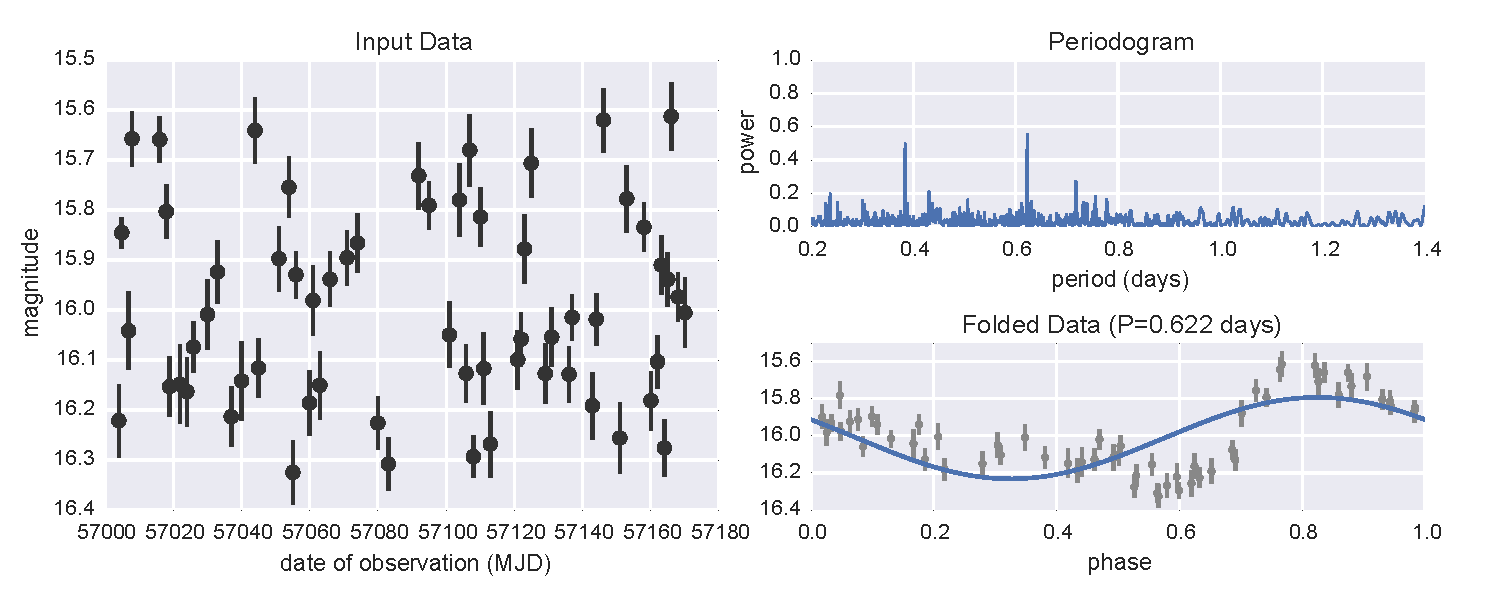
\includegraphics[width=\textwidth]{fig01.pdf}
  \caption{
    An illustration of the basic periodogram and its relationship to the single-term sinusoid model. The left panel shows the input data, while the right panels show the fit derived from the data. The top-right panel shows the periodogram, showing a distinct peak at the true period of 0.622 days, and the bottom-right panel shows the data as a function of phase as defined by this period. Note in the periodogram the presence of the typical aliasing effect, with power located at beat frequencies between the true period and the 1-day observing cadence (see \sect{simple_period} for further discussion).
  }
  \figlabel{basic_example}
\end{figure}

In the upper right, we see the normalized periodogram as a function of period. While the power does peak at the true period of 0.622 days, an aliasing effect is apparent. These additional peaks are due to beat frequencies between the true period $P$ and the observing cadence of $\sim 1$ day. That is, for nightly observations, we'd expect excess power to be found at frequencies $P / (1 + nP)$ for a positive or negative integer $n$. This explains the prominent peak at $0.383$. For the current work, we'll ignore this (important) piece of the period-finding problem; for a thorough discussion of aliasing within astronomical time series, see \citet{Roberts87}.

The lower-right panel shows the maximum likelihood interpretation of this periodogram: it is a measure of the normalized $\chi^2$ for a single-term sinusoidal model. Here we visualize the data from the left panel, but folded as a function of phase with the best-fit single-term model over-plot. Here its apparent that the single-term model is biased: RR Lyrae are much more complicated than a simple sinusoid. Nevertheless, the simplistic sinusoidal model does well to zero-in

\subsubsection{Discussion}
We have shown two forms of the classic normalized periodogram: \eq{LombScargle} and \eq{LombScargle2}. Though the two expressions are equivalent, they each have distinct advantages. The expression in \eq{LombScargle} avoids the explicit construction of a matrix, and thus can be computed very efficiently. In particular, through some computational tricks involving the FFT, expressions of the form of \eq{LombScargle} can be evaluated for $N$ frequencies in $\mathcal{O}[\log{N}]$ time \citep{Press89}.

The matrix-based formulation of \eq{LombScargle2} sacrifices some potential computational efficiency in order to attain several advantages:
\begin{enumerate}
  \item It is trivially extended to heteroscedastic and/or correlated measurement noise in the data $y_k$ through appropriate modification of the noise matrix $\Sigma$
  \item It is trivially extended to more sophisticated linear models by appropriately modifying the design matrix $X_\omega$.
  \item It is trivially extended to L2-regularized likelihoods by adding an appropriate diagonal term to the normal matrix $X_\omega^T\Sigma^{-1}X_\omega$.
\end{enumerate}
In the remainder of this section, we'll explore a few of these modifications.


\subsection{Stationary Sinusoid with Floating Mean}
\sectlabel{floating_mean}

\begin{figure}
  \centering
  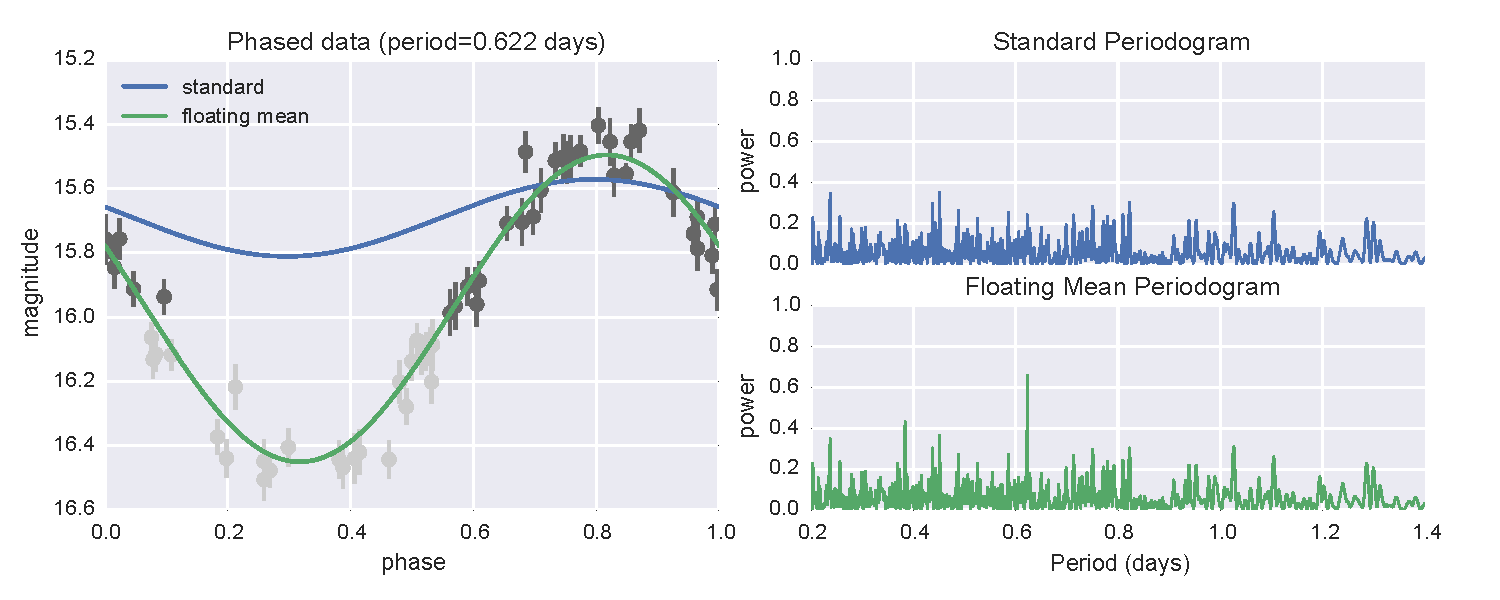
\includegraphics[width=\textwidth]{fig02.pdf}
  \caption{
    An illustration of the effect of the floating mean model for biased data.
    The data consist of 80 observations drawn from a sinusoidal model; all observations with magnitude fainter than 16 are masked, as shown in the left panel. The standard and floating-mean periodograms are computed from the unmasked data; these are shown in the right panel. Because of this biased observing pattern, the mean of the observed data is not a good predictor of the true mean, and the standard model fails to recover the true period of 0.622 days, while the floating mean model still finds the correct period.
  }
  \figlabel{floating_mean}
\end{figure}

As an example of one of these generalizations, consider the {\it generalized Lomb-Scargle} method of \citet{Zechmeister09}. This adjusts the classic Lomb-Scargle algorithm by using a model with a floating mean, which can be more accurate for certain observing cadences:

\begin{equation}
  y(t~|~\omega, \theta) = \theta_0 + \theta_1\sin\omega t + \theta_2\cos\omega t
\end{equation}

While \citet{Zechmeister09} details a formalism to express this floating-mean model (which they call a ``generalized periodogram'') similarly to \eq{LombScargle}, in the matrix formalism all that is required is to add a column of ones to the $X_\omega$ matrix before computing the power via \eq{LombScargle2}.

For well-sampled data, there is little difference between a standard periodogram and a floating-mean periodogram. Where this becomes important is if selection effects or observing cadences cause there to be preferentially more observations at certain phases: an example of this situation is shown in \fig{floating_mean}. The data are drawn from a sinusoid with Gaussian errors, and data with a magnitude fainter than 16 are removed to simulate an observational bias. Because of this bias, the mean of the observed data to be a poor predictor of the true mean, which makes it so that the standard approach fails to find a suitable fit to the data. The floating-mean approach is able to adjust for this, resulting in a periodogram which detects the input period of 0.622 days.

\subsection{Truncated Fourier Models}
\sectlabel{multiterm}

\begin{figure}
  \centering
  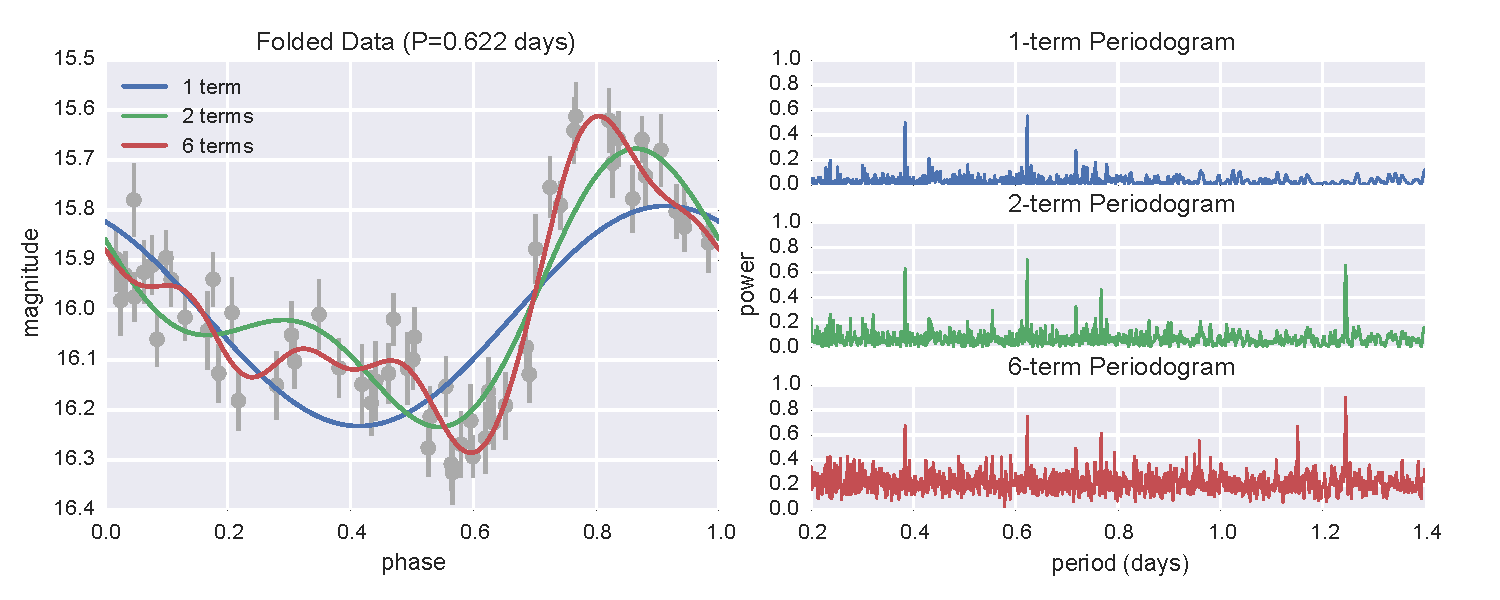
\includegraphics[width=\textwidth]{fig03.pdf}
  \caption{
    An illustration of a periodogram based on the truncated Fourier model. The data are the same as those in \fig{basic_example}. 
  }
  \figlabel{multiterm_example}
\end{figure}

The classic Lomb-Scargle approach is equivalent to fitting a single-term stationary sinusoidal model to the data. A natural extension is to use a multiple-term sinusoidal model. With $M$ terms, there are $2M + 1$ free parameters, and the model is given by:

\begin{equation}
  y(t|\omega,\theta) = \theta_0 + \sum_{n=1}^M \left[\theta_{2n - 1}\sin(n\omega t) + \theta_{2n}\cos(n\omega t)\right]
\end{equation}

Because this remains a linear model, it can be easily accommodated into the matrix formalism above. For example, an $M = 2$-term model can be constructed by building a design matrix $X_\omega$ with $2M + 1 = 5$ columns:

\begin{equation}
X_\omega^{(2)} = \left[
\begin{array}{ccccc}
1 & \sin(\omega t_1) & \cos(\omega t_1) & \sin(2\omega t_1) & \cos(2\omega t_1)\\
1 & \sin(\omega t_2) & \cos(\omega t_2) & \sin(2\omega t_2) & \cos(2\omega t_2)\\
1 & \sin(\omega t_3) & \cos(\omega t_3) & \sin(2\omega t_3) & \cos(2\omega t_3)\\
\vdots & \vdots & \vdots & \vdots & \vdots \\
1 & \sin(\omega t_N) & \cos(\omega t_N) & \sin(2\omega t_N) & \cos(2\omega t_N)\\
\end{array}
\right]
\end{equation}
Using $X_\omega^{(2)}$ in \eq{LombScargle2} will result in a two-term periodogram. In general, we can fit an $M$-term periodogram by simply adding terms to the fit. \fig{multiterm_example} shows a few examples of this multiterm Fourier approach as applied to a simulated RR Lyrae light curve constructed from templates derived in \citet{Sesar2010}. There are several important features of this figure that give us insight into the subtleties of this type of fit:

First, we see in the right panel that all three models show a significant spike at the true period of $P_0 = 0.622$. The higher-order models, however, also show a a spike of poer at $P_1 = 2 P_0$: the reason for this is that the fundamental model of the single-term model at $P_0$ is the first harmonic of the 2-term model at $2P_0$, so the higher-order models contain this single-term result.

Second, notice that as the number of terms is increased, the general ``background'' level of the periodogram increases. This is due to the fact that the periodogram is directly related to the $\chi^2$ of the fit. A more complicated model will have the flexibility to conform to the data at {\it all frequencies}, and thus the observed ``power'' is stronger at all frequencies.

\subsection{Regularized Models}
\sectlabel{regularization}
The previous sections raise the question: how complicated a model should we use? If we added many terms to the truncated Fourier series, we might fit the data perfectly, but eventually we would {\it overfit} the data: that is, our model is fitting the noise rather than the signal. This can be avoided by explicitly truncating the series, but another approach is to use a {\it regularization} term to enforce a less complicated model.

A regularization term is an explicit penalty on the magnitude of the model parameters $\theta$, and can take any number of forms. For computational simplicity here we'll use an {\it L2 regularization} (also known as Tikhonov Regularization), which is a quadratic penalty term in the model parameters. This is mathematically equivalent to the Bayesian approach of using a Gaussian prior on the model parameters.

We'll encode our regularization in the matrix $\Lambda = {\rm diag}([\lambda_1, \lambda_2 \cdots \lambda_M])$ for a model with $M$ parameters, and our expression for $\chi^2$ becomes
\begin{equation}
  \eqlabel{chi2reg}
  \chi_\Lambda^2(\omega) = (y - X_\omega\theta)^T\Sigma^{-1}(y - X_\omega\theta) + \theta^T\Lambda\theta
\end{equation}
Minimizing this $\chi^2$, solving for $\theta$, and plugging into the expression for $P_N$ gives us the regularized counterpart of \eq{LombScargle2}:
\begin{equation}
  \eqlabel{LombScargleReg}
  P_N(\omega) = \frac{y^T\Sigma^{-1}X_\omega~[X_\omega^T\Sigma^{-1}X_\omega + \Lambda]^{-1}~X_\omega^T\Sigma^{-1}y}{y^T\Sigma^{-1}y}.
\end{equation}
Note that the effect of this regularization term is to add a diagonal term to the normal matrix $X_\omega^T\Sigma^{-1}X_\omega$, which has the additional feature that it corrects ill-posed models. This feature of the regularization will become important below.

\todo{Show a regularized model?}

\section{Moving to Multiple Bands}

To compute a periodogram for multi-band data, we'll take advantage of many of the nice features of the matrix form of the normalized periodogram, which allows us to specify an arbitrary linear model covering our data. We will construct a multi-term Fourier model with the following features:
\begin{enumerate}
  \item An $M_{base}$-term truncated Fourier fit which models a latent parameter, which we'll call the ``overall variability''.
  \item An $M_{band}$-term truncated Fourier fit which models the residual of each band from the overall variability.
\end{enumerate}
The total number of parameters for $N_{filt}$ filters is then $M = (2M_{base} + 1) + N_{filt}(2M_{band} + 1)$. The model looks as follows, for a band $b$:
\begin{eqnarray}
  y(t|\omega,\theta,b) = &&\theta_0 + \sum_{n=1}^{M_{base}} \left[\theta_{2n - 1}\sin(n\omega t) + \theta_{2n}\cos(n\omega t)\right]\\ 
  &+& \theta^{(b)}_0 + \sum_{n=1}^{M_{band}} \left[\theta^{(b)}_{2n - 1}\sin(n\omega t) + \theta^{(b)}_{2n}\cos(n\omega t)\right].
\end{eqnarray}
The important feature is that {\it all bands} share the same base parameters $\theta$, while their offsets $\theta^{(b)}$ are fit within each band.

We can build the matrix form of this model by building a sparse $X_{\omega}$ matrix with $M$ columns. Each row corresponds to a single observation through a single band; columns corresponding to the base model and the observation band will have nonzero entries; all other columns will be filled with zeros. For example, the $X_\omega$ matrix with $N_{base}=1$ and $N_{band}=0$ (that is, a single sinusoid model with independent offsets to each band) will look as follows:

\begin{equation}
X_\omega^{(1,0)} = \left[
\begin{array}{cccccccc}
1 & \sin(\omega t_1) & \cos(\omega t_1) & 1 & 0 & 0 & 0 & 0\\
1 & \sin(\omega t_2) & \cos(\omega t_2) & 0 & 1 & 0 & 0 & 0\\
1 & \sin(\omega t_3) & \cos(\omega t_3) & 1 & 0 & 0 & 0 & 0\\
1 & \sin(\omega t_4) & \cos(\omega t_4) & 0 & 0 & 1 & 0 & 0\\
\vdots & \vdots & \vdots & & & \vdots & &\\
1 & \sin(\omega t_N) & \cos(\omega t_N) & 0 & 0 & 0 & 0 & 1\\
\end{array}
\right]
\end{equation}
Here the structure of the final five columns indicates the band observed at the given time: the first row is a $u$-band measurement, the second is a $g$-band, the third is a $u$-band, etc.

From reasoning about the free parameters, or by examining the above matrix it is easy to see that some of the parameters will be degenerate (i.e. $X_\omega$ is low-rank). Intuitively, this is due to the fact that if we add an overall offset to the base model, this can be perfectly accounted for by subtracting that same offset from each of the band columns. In order to proceed, then, we'll either have to correct this model deficiency, or use a regularization term on one of the offending parameters. We'll choose the latter here, and regularize all the band columns to drive the common behavior into the base model. For the above matrix,
this regularization will look like
\begin{equation}
  \Lambda = {\rm diag}([0, 0, 0, \epsilon, \epsilon, \epsilon, \epsilon, \epsilon])
\end{equation}
where $\epsilon$ is some small fraction of the trace of the matrix $[X_\omega^T\Sigma^{-1}X_\omega]$. With this regularization in place, the model is well-posed and \eq{LombScargleReg} can be used to straightforwardly compute the power. We'll see an example of this in action in \sect{Simulated}.

\todo{Talk about the $N_{base} = 0$, $N_{band} = 1$ case. This is equivalent to fitting a floating-mean Lomb-Scargle independently to each band, and constructing a weighted sum of each individual periodogram.}

\section{Examples}
Here we'll show several examples of the multiband periodogram method in action.

\subsection{Simulated Example}
\sectlabel{Simulated}

\begin{figure}
  \centering
  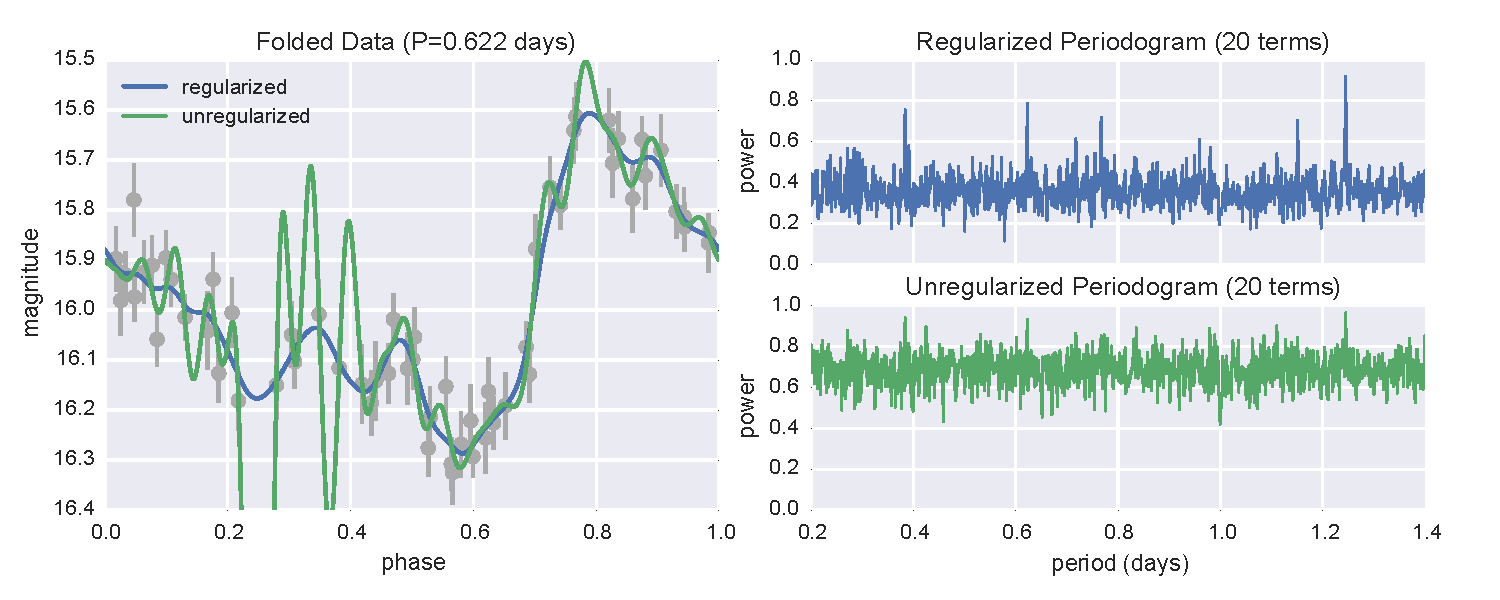
\includegraphics[width=\textwidth]{fig04.pdf}
  \caption{
    An illustration of the typical approach to multiband periodograms,
    in which each band is fit individually. The data consists of 60 coeval
    {\it ugriz} observations spread over 180 nights, and is based on an
    RR Lyrae template from \citet{Sesar2010}. With this much data in each
    band, individual periodograms can be constructed and compared to find the
    true period $P=0.622$ days
  }
  \figlabel{adhoc_example}
\end{figure}

\fig{adhoc_example} shows a simulated RR Lyrae light curve based on a template from \citet{Sesar2010}. The observations take place on 60 random nights over a 6-month period, and each night all five bands ({\it u,g,r,i,z}) are recorded. The left panel of \fig{adhoc_example} shows the observations folded as a function of phase.
Using the typical approach from the literature prior to this paper, we individually compute the Lomb-Scargle periodogram within each band: the results are shown in the right panel. Here the data is well-enough sampled that a distinct period of 0.622 days can be recognized within each individual band.\footnote{\label{foot1}
  An aliasing effect is readily apparent in the left panel of \fig{adhoc_example}: these additional peaks are due to beat frequencies between the true period $P$ and the observing cadence of $\sim 1$ day. That is, for nightly observations, we'd expect excess power to be found at frequencies $P / (1 + nP)$ for a positive or negative integer $n$. For the current work, we'll ignore this (important) piece of the problem; for a thorough discussion of aliasing within astronomical time series, see \citet{Roberts87}.}


\begin{figure}
  \centering
  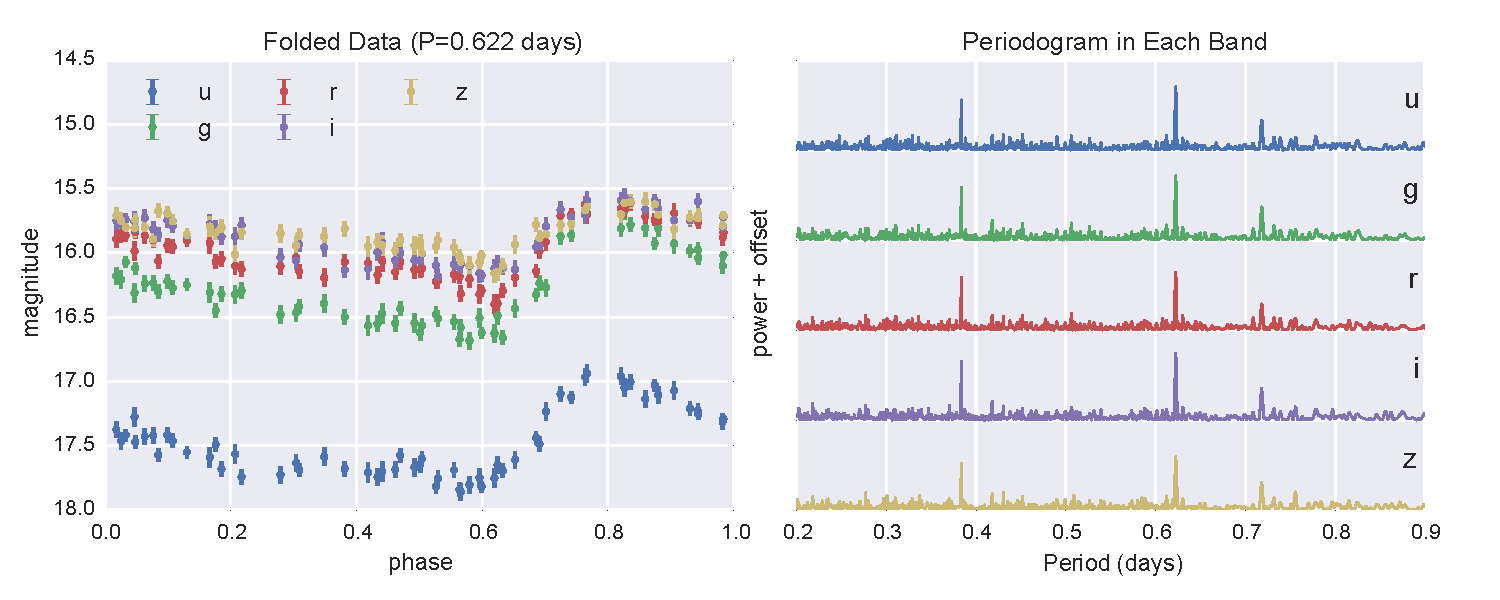
\includegraphics[width=\textwidth]{fig05.pdf}
  \caption{
    Another realization of the data from \fig{adhoc_example}, with only a single
    band observed each night (i.e. 12 observations per band, spread over 180
    days). In this case, single-band data is not sufficient to recover the
    Lomb-Scargle peaks, and the classic band-by-band approach fails.
    By utilizing all the data at once with the multiband approach
    (with $N_{base}=1,~N_{band}=0$),
    we faithfully reconstruct the periodogram and recover
    the dominant power at period $P=0.622$ days.
  } 
  \figlabel{multi_example}
\end{figure}

\fig{multi_example} shows the same 60 nights of data, except that each night only a {\it single} band observation is recorded. The left panel again shows the observations as a function of phase, and the right panel shows the Lomb-Scargle fits to the data. Now, with only 12 observations for each indiviudal band, there is not enough data to accurately determine the period band-by-band. With the multiband approach (here computed for $N_{base}=1$ and $N_{band}=0$), as seen in the lower-right panel of \fig{multi_example}, the period is cleanly recovered.


\subsection{Stripe 82}

\begin{itemize}
  \item Compute periods using majority method
  \item Compute periods using unified method
  \item Compare the results
\end{itemize}

\section{Discussion and Conclusion}

\subsection{Further Study}
\begin{itemize}
  \item issues with aliasing \& window function corrections
  \item issues with physicality of model
\end{itemize}


\bibliographystyle{apj}
\bibliography{paper}

%\appendix

\end{document}
